%************************************************
\chapter[Modelling]{Modelling}\label{ch:Modelling}
%************************************************

\begin{flushright}{\slshape the sciences do not try to explain, they hardly even try to interpret, they mainly make models. By a model is meant a mathematical construct which, with the addition of certain verbal interpretations, describes observed phenomena.} \\ \medskip
    --- John  von Neumann
\end{flushright}

As said by von Neumann, science is about making models. They can be used to simplify a phenomena and make it easier to understand and define, moreover, a model can be used to quantify or visualise reality. Knowledge extracted by the process of modelling can be reused to create a simulation (\ie, another form of modelling) of the system under analysis. For all these reasons, and because is one of the most innate ability of humans, modelling has always been the cornerstone of science, engineering and arts.

Modelling in engineering is an essential tool for design, analysis and simulation, models have different characteristics and take various shapes. A collection of mathematical formulas can be used to describe a physical phenomena (\eg, friction between the ground and the wheels), or the behaviour of a system (\eg, a control system). Differently, a flow chart is a graphical model of an execution process, while pseudo-code is a textual one. A 3D model capture the physical shape of an object and can be used to study the design or the space occupancy.

This chapter presents various modelling techniques that we used to describe multiple aspect of the architecture of a robot. First, we introduce the \textit{component-and-connector} paradigm, its basic concepts and why it is used in robotics. From there, we move to the AADL representation of the paradigm, and an extension to cover first a ROS node and later a complete architecture. To conclude the description on modelling robotic system, we introduce a series of template to simplify the modelling process. Lastly, since AADL is not a data modelling language, we present two approaches based on Abstract Syntax Notation One (ASN.1) and JavaScript Object Notation (JSON) to model the data exchanged in the system (\ie, ROS messages) and the internal state of each component.

\minitoc
\newpage

\section[The component and connector paradigm]{The component and connector \\paradigm}
\label{sec:cnc}
In robotics, the most popular middlewares and frameworks are based on a \textit{component-and-connector} paradigm, while different approaches implement it in different ways, the underlying conceptual structure is the same. In ROS, it is represented by the computation graph, a peer-to-peer network of processes managing and exchanging data together. Here, following the usual terminology of graphs, the components are called nodes, while the connections are represented by asynchronous topics or synchronous services; in both cases the communication happens by exchanging messages. In SmartSoft, the underlying technological approach of the SmartMDSD toolchain, the structure is based on components, communication patterns and communication objects. Components are interconnected to each other by using one of the four possible communication patterns: two synchronous based on a client/server paradigm (\ie, send and query) and two asynchronous based on a publisher/subscriber paradigm (\ie, push and event). All the patterns communicate by exchanging communication objects. Another example is the Robot Construction Kit (RoCK), which is based on the component model of the Orocos Real Time Toolkit (RTT). In RoCK, and consequentially in Orocos, the architecture is, again, based on components connected to each other through ports. One last example is the OpenRTM-aist middleware developed by the Japanese National Institute of Advanced Industrial Science and Technology. They fully embraced the component based approach, where a robot is made by multiple subsystem, and each of them is a collection of components. Components communicate to each other using connections established between predefined ports. The popularity of the \textit{component-and-connector} paradigm is not coincidental. In their structure, robots are a system of systems, a hierarchical collection of components interconnected together to create a working apparatus. Physically, a robot is a collection of sensors and actuators; same goes for the behaviour, simple low-level independent functionalities are not enough to implement even the simplest robot. Given all these needs, the most natural approach is to decompose the system in different and simpler subsystems and to simplify and characterise their interactions by the use of interfaces; the result is a \textit{component-and-connector} paradigm. 

The aim of this work is to provide a general and flexible representation that can be used to model an architecture that captures the design a robot and it is compatible, at least at an higher level of specification, with multiple middlewares and frameworks. To do so, we defined some common design patterns often used when creating robotic architectures. As already mentioned, the first key design approach is the use of components and connections, but, of course, this is a very high-level description and it is only useful to define the topology. To better define an architecture without including technological details (\ie, specify a middleware or framework), we have to define a general description for component functionalities and we have to specify the nature of each connection. By analysing the existing solutions for robotics (\ie, ROS, SmartSoft and Orocos/RoCK), we identified four possible component behaviours that can exist (and coexist) in a component.

\paragraph{Source} A component expresses a \textit{source} behaviour when it is a generator of data or events. An example is a simple ROS node implementing a publisher, it generates messages and circulates them in the computational graph. In SmartSoft there are two communication patterns that, implemented in a component, evoke this behaviour: push, to generate message and send them to other components, and event, a data-less communication to trigger action in other components. This type of behaviour is used for device drivers, since they create and circulate a digital version of the analogue input they detect, but also it used by coordinator components, they are in charge of initiating high level functionalities by generating an event or a specific message.

\paragraph{Sink} A \textit{sink} is a component that consumes data or events. In ROS, a node is a sink when it implements a subscriber that receives, processes, and consumes messages. The counterpart in SmartSoft is, again, a component that implements the same two communication patterns (\ie, push and event), but this time it is on the receiving side of messages and events. This type of behaviour is implemented by component controlling actuators, they receive commands from other components and consume them to operate a physical device. Alternatively, it is used by storage managers or loggers, they simply collect all possible messages and store them. Lastly, any component activated by an event implements a corresponding \textit{sink} to receive and mange the trigger.

\paragraph{Filter} The most common behaviour for a component is the \textit{filter}. This type of component receives messages or events as an input and processes or relays them to the create an output. To describe more precisely the internal functioning of this behaviour, we have to distinguish two categories: without or with memory. 

In the former, the component does not store in any way the data received, they are processed and directly re-circulated in the system. This approach is common when doing simple conversions (\eg, change the unit of measurement or the coordinate system) or when it is necessary to resample the data (\eg, change the frequency or zero-pad the messages). In ROS, it is implemented by processing the received message directly in the subscriber callback and publish it before the leaving the callback environment. The latter behaves similarly to a combination of a \textit{sink} and a \textit{source}; messages or events are received by the component and stored locally, then, at a later time, recalled from memory, processed and relayed in the system. This approach is used when doing more complex processing, for example when multiple messages need to be processed at the same time (\eg, smoothing a velocity set-point), or when multiple inputs need to converge in a single output (\eg, combining multiple laser rangefinder measurements in a single one). In ROS, this happens when messages are processed in a callback but not completely discarded at the end, and later, in the main loop or in a different callback, they are processed and circulated back in the computational graph.

\paragraph{Reactive} A component has a \textit{reactive} behaviour when its functionalities are synchronously triggered by a message or an event, it is usually implemented by using a remote function call. In ROS this kind of behaviour is exemplified by services; they offer a public interface that can be called by external components and react with a synchronous execution of a function that may return a value.  SmartSoft implements a similar synchronous system, but differentiate between a one way communication with no answer (\ie, send and forget) and a two way communication with a specific response. This behaviour is used to delegate to a central component a specific functionality (\eg, centralised conversion system), to activate a remote functionality (\eg, component \mbox{re-initialization}), or to guarantee a timely answer to a request (\eg, soft real time functionalities).

Implicitly, by describing the possible behaviours of a component, we already outlined the nature of the messages exchanged: a connection can be data-based or event-based. In a data-based connection, messages with a specific content are exchanged between components. Usually, a specific communication channel only support a pre-defined data format, but, in theory, it is possible for a data-based connection to not specify the nature of the message exchanged. Each middleware or framework uses a different language to describe data format, for example both ROS  and SmartSoft use their own domain specific language to define communication objects. This is source of a strong and unnecessary fragmentation, because in the end all middlewares and frameworks rely on basic data types and data structures, that are already covered by numerous standard data description languages. Event-based connections fall on the opposite side of the spectrum, since there is no data exchanged, the key element is the communication itself. The receiver only needs to detect an active connection to collect the event generated by the sender. In practices, it is common to implement event-based communications as data-based communication carrying an empty message, this is the approach used by ROS, since it doesn't support any pure event-only communication, but any communication channel (\ie, topics and services) supports standard empty messages. In SmartSoft, event-based communication is supported only paired with a publish/subscribe paradigm, since the \textit{Event} communication pattern exists only for asynchronous communications.

The complete the description of an architecture based on the \textit{component-and-connector} paradigm, we need to analyse the cardinality of the connections. Potentially, there are four different cardinality:
\begin{itemize}
\item \textit{1-1}, this is an exclusive connection where the a source is directly connected to exactly one destination.
\item \textit{1-n}, in this type of connection the stream of messages or events generated by a single source can be connected to one or multiple destinations.
\item \textit{n-1}, to achieve this configuration multiple sources need to converge in a single destination.
\item \textit{n-n}, this is the most permissive of all cardinalities. In this configuration there is no limit in the number of sources and destinations for a single communication channel. By using a local policy to this type of communication it is possible to implement all the previous ones, however when a communication is \textit{n-n} by design it is impossible to guarantee other cardinalities. The result is a very flexible, yet unpredictable connection.
\end{itemize}
In practice, robotic middlewares and frameworks, rarely implement all four options. In ROS, topics are implemented as pure \textit{n-n} communication channels, since they follow a \textit{publish-and-forget} paradigm. Any number of publishers can publish messages on a topic and each subscriber receive a copy of the message. There is no ownership of a messages after it is published on a topic. While the communication supports a full \textit{n-n} cardinality, in practice, it is never used as such, but always as multiple publisher and a single subscriber (\ie, \textit{n-1}) or a single publisher and multiple subscribers (\ie, \textit{1-n}). ROS services are inherently \textit{n-1}, since only a single server can provide a specific service, while multiple clients can request it. SmartSoft is more strict in the definition of the cardinality of its communication patterns: all the patterns with a publish/subscribe structure (\ie, push and event) have a \textit{1-n} cardinality, all the patterns following a client/server approach (\ie, query and send) support only a \textit{n-1} cardinality.

\section{AADL for robotics}
\label{sec:aadl-robot}
The Architecture Analysis \& Design Language was originally developed in the field of avionics, then it was redesigned to target embedded real-time systems; therefore, never in its history the language was specifically designed for robotics. However, a lot of parallels exists between embedded and robotics systems, consequentially, characteristics that were designed for the former are more than suitable for the latter. Moreover, a general design approach means the language is not bound to a specific field and its design was not conditioned by the existing methodologies and technologies. Its agnostic nature makes AADL an excellent choice to provide a general modelling language for robotic systems, different middlewares and frameworks sharing similar design principles can be represented easily with a common language. Additionally, AADL formal syntax and expressiveness guarantee consistency in the models and reduce the necessity to introduce extensions and ad hoc modifications, and even when this is necessary, they are regulated by the language itself.

%TODO rephrase section to chapter
As described in Chapter~\ref{ch:AADL}, AADL provides modelling tools for both hardware and software components. This is expected from a modelling language designed for embedded systems, where the development of the software components is tied to the hardware platform, however, this characteristic is extremely useful for robotics, too. Thanks to the abstraction provided by component-based middlewares, modern robotic systems are not tightly connected to the underlying hardware platform as they used to be; today an obstacle avoidance system does not need to know exactly the data format of the measurements provided by the laser rangefinder to work correctly. However, this is true only for the development of single components or compartmentalised set of components, when designing the whole system or during execution, it is necessary to take in account the behaviour of both hardware and software. \textit{How many and which sensors the robot uses to localise itself? Is there a teleoperation system? How much time it takes for a measurement to propagate in the system? How many critical functionalities are interrupted by a faulty sensor or actuator?} All these critical questions have to be answered during the design phase of the system, and this can be done by correctly modelling the hardware (sensors, actuators, connections, execution platforms, \etc), the software (drivers, low-level interfaces, functionalities, \etc), and their interactions.

In AADL, a designer can use properties to specify the finer characteristics of each component. Some examples are memory size, processors computational power, processes resource consumption, or connection throughput. All these properties can be used to perform a formal analysis of the system before deployment, or even before the implementation. One of the tools provided by AADL is the concept of flow, they are logical path through the architecture and they are specified from a component input to a component output. These flows can go through any type of feature (\ie, ports, accesses, groups and abstracts) and can represent any logical pathway (\eg, data, control, fault event, \etc). When modelling a flow, it is necessary to specify the source, the sink and the complete path of the flow, however, the definition can be done at system-level, it is not necessary to specify the behaviour of the flow inside the components. From this specification, it is possible to do end-to-end analysis, for example, identify the component involved in a critical communication, estimate error propagation, calculate the time necessary for a measurement to impact on the behaviour of an actuator. Information and analysis about propagation time of messages and latency are fundamental in hard real-time application, but even soft real-time application can benefit from a strict performance analysis. For example, an high-speed delta robot need to consider communication latency to operate with high precision, or in an autonomous wheelchair, while the control system doesn't need high reactivity given the speed involved, a correct estimation of the latency will make the difference between a sudden braking and a gentle slowdown when faced with an unexpected obstacle.

On a more technological level, the detailed description of components, their interactions, their structure and hierarchy provided by AADL is extremely useful to solve some intrinsic problems of robotic middlewares. For example, if we consider ROS, there is a total absence of an architectural view of the system. A partial representation of the interactions of the components is available at runtime by using tools like \texttt{rqt\_graph}, but this representation only consider topics and does not reflect the full structure of the system. Something similar can be achieved during deployment by using launch files, but while they are useful to organise the runtime of the components, there is no way to visualise the interactions between them and they do not capture the internal connections. Both this limitations can be solved by using AADL, a complete model of the architecture provides a view of the system since its inception and by using the \textit{system} component is possible to recreate the same hierarchy provided by launch files. Even when considering middlewares more focused on a model based approach, AADL can bring great advantage. In the SmartMDSD toolchain, architectures are designed using a custom meta-model defined via the Eclipse Modelling Framework, this approach limits the design process to a very specific environment and tightly connects the design phase with the implementation phase, since the model reflect exactly some specific software artefacts. Moreover, while quite complete, the SmartMDSD meta-model, do not consider the hardware components as part of the architecture, therefore any analysis related to the hardware has to be done with additional tools. In this case, AADL could be used as a general high-level modelling language compatible with the SmartMDSD meta-model, to be then transformed in an intermediate representation compatible with the existing code generators. The AADL version of the model could be used to perform analysis and to speculate on the possibility of using different technologies to implement different components, or to deploy the same design on different platforms.

While not strictly related with robotics, an important feature of the language is the active community, and the available tools. The Open Source AADL Tool Environment (OSATE) is a development environment not only to develop AADL models both graphically and textually, but also to exploit all the validation and analysis capabilities of the language. Some examples are: end-to-end latency analysis, port connections consistency checks, computer resources budget analysis. Moreover, OSATE act as an interface for the capabilities provided by Ocarina, an AADL model processor that supports parsing, code generation and model checking. Ocarina uses a front end/back end paradigm, where the front end is the AADL parser and a back end can be any code generator that goes from the intermediate representation provided by the front end to an executable code. Ocarina already support various targets for code generation, none of these is a robotic middleware, however, thanks to the front end/back end paradigm, we created a suitable code generator that goes from an AADL model to a complete ROS architecture. This code generation process will be described in details in Chapter~\ref{ch:code-gen}.

\subsection{Modelling the C/C paradigm in AADL}
\label{sec:aadl-cnc}
AADL is the perfect candidate to describe architectures based on this paradigm, because the language itself, while centred around the concept of schedulability of threads, is designed to support the structure defined by components and connections. AADL components, at any level (\eg, system, process, device, subprogram, \etc) support, some form of feature (\ie, ports and accesses) to communicate and interact with other components. In the previous section we described all the elements useful to characterise the robotic components and their interactions (\ie, component behaviours, type and cardinality of connections), in this section we will describe how the same concept can be modelled by using AADL.

First of all, it is necessary to outline which AADL artefacts are necessary to model this kind of paradigm. As described in Chapter~\ref{ch:AADL}, the general top level container is the \textit{system} category, one step below there are three possible software categories that could act as components: \textit{process}, \textit{data} and \textit{subprogram}. A collection of subprograms as subcomponent of a system is used to model libraries or sets of APIs, data as first level subcomponents model general storage or shared resources, processes are used to describe an enclosed execution space and can exist only as direct subcomponents of a system. Therefore, it is clear that the perfect candidate to model components in the \textit{component-and-connector} paradigm is the \textit{process} category. Since the execution space of a process is directly accessible only by its own subcomponents, the category supports, on its frontier, all available AADL features (\ie, interfaces). 

We described in the previous section how communication can be data or event based, AADL supports both this types of communication thanks to the additional type specifier when defining a feature, it can be a \textit{data port}, an \textit{event port} or an \textit{event data port}. Moreover, ports can be characterised by a specific data type, defined using a \textit{data} category, this is useful to model the type of message exchanged in the connection. In AADL, all ports have natively a \textit{n-n} cardinality, with the exception of the \textit{input data port}; since this type of port models a communication with no queue, it does not support multiple incoming connections, however they are supported by the \textit{input event data port} since it includes a queue in its model. In the base language, there is no way of restricting the cardinality of ports, but it is possible to define extra properties to better specify a connection and, eventually, indicate its cardinality.

To model component behaviours, it is necessary to go a step further in the component hierarchy and to take in account the potential subcomponents of a process. Again, the \textit{data} and \textit{subprogram} categories are potential subcomponents, but are not relevant to describe the behaviour of a component, since they are used to define memory and subroutines. The third, and more suitable, candidate is the \textit{thread} category. They represent an execution path through code and their execution behaviour is periodic with various characteristics or triggered by an external input (\eg, incoming data or events), moreover, multiple threads can coexist in the same process and, potentially, execute in parallel. All this characteristics make the thread a suitable category to model component behaviours. However, as we described in the previous section, each behaviour is related to a specific interaction outside the frontier of the component, therefore to completely characterise it, it is necessary to combine a thread with a specific port.
\paragraph{Source} In this behaviour the components generates messages or events. Therefore the thread needs an output port that can be of type data or event. Since there is no external source triggering this behaviour, it is necessary to specify the scheduling of the thread, usually periodic.
\paragraph{Sink} In this case the components receives and consumes messages or events. Given this, an input port needs to be modelled as interface of the thread. By changing the type of the input port it is possible to change the how the sink behave. A data port, combined with a periodic scheduling, would model a sampler that receive a constant stream of data, an event data port would define the subscriber of a publish/subscribe paradigm, an event port defines a sink managing external triggers.
\paragraph{Filter with memory} For this type of behaviour it is necessary to add the extra memory element, in AADL all memory, on a software level, is modelled using the \textit{data} category. Therefore, to completely model this type of filter, it is necessary to define a data component inside the process that acts as a shared memory between two threads, one with a input port (\ie, sink equivalent) and one with an output port (\ie, source equivalent).
\paragraph{Filter without memory} This type of filter is easier to model, since there are less elements. All processing happens directly in the thread that receive the message and the same thread is responsible to circulate it back in the architecture. Given this, this behaviour is modelled using a single thread with an input port of any kind and a corresponding output port.
\paragraph{Reactive} This behaviour represents a synchronous remote execution similar to a remote function call. In AADL there are various approaches to model a RFC, to keep the structure more in line with the other behaviours the best option is to pair a thread with a remote subprogram call. To do so, it is necessary to define a \textit{subprogram} as a subcomponent of a thread and, on the frontier, declare an access bound to that specific subprogram.

\begin{figure}[t]
    \centering
    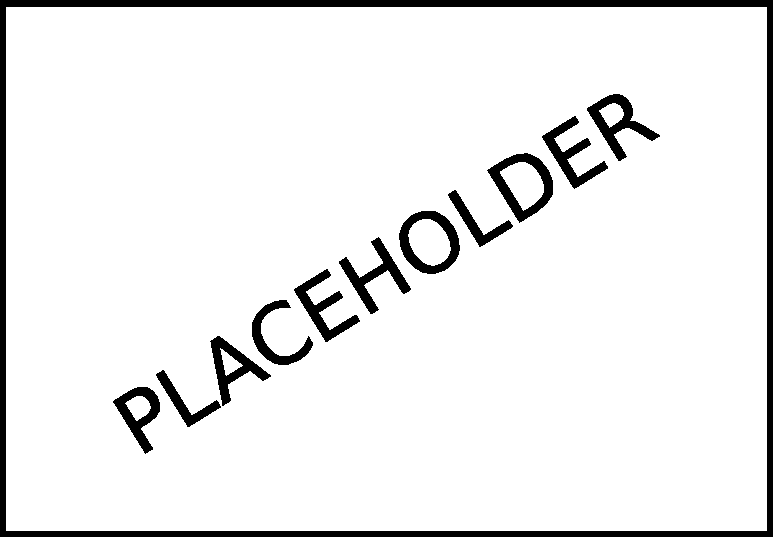
\includegraphics[width=0.8\textwidth]{gfx/placeholder}
    \caption{TODO}\label{fig:cnc-arch}
\end{figure}

\subsection{A basic example}
\label{sec:cnc-basic}
With the paradigm described in Section~\ref{sec:cnc} and the tool provided by AADL presented in Section~\ref{sec:aadl-cnc}, it is possible to define a basic architecture, not only the topology of the connections, but also the internal functioning of the components. As an example, let us take the architecture defined in Figure~\ref{fig:cnc-arch}; in this simple architecture we want to model a robot with two control functionalities: line following and teleoperation.

In the top branch of the architecture we have the line following subsystem: a sensor driver that generates measurements indicating the presence of a black line on the ground and a simple component that directly translate the sensor input in a velocity command. The former expresses a \textit{source} behaviour, it generates messages and circulates them in the system, it is modelled by a process containing a periodic thread, on the frontier there is a output data port. The latter has a \textit{filter} behaviour, it has two ports on its frontier: one input event data port, to queue the messages and trigger a functionality of the component, and one output data port, to send to the next component the velocity commands. In this example, the line following component is very simple and can estimate a set-point directly from the sensor measurements, this means that it does not need to store any information: it is a filter without memory. The internal model of the components is a single thread with an input and an output port, both directly connected to their corresponding ports on the process frontier.

On the bottom branch there is the teleoperation subsystem: a joypad driver providing readings of the input and a teleoperation component to convert the joypad input in set-points. Similarly as the other branch, the driver expresses a \textit{source} behaviour, it converts the input coming from the joypad in messages compatible with the architecture. The teleoperation component, however, does not have the same \textit{filter} behaviour of the line follower, since it stores the incoming messages to smooth the set-point: it is a filter with memory. To model it, it is necessary to define on the frontier of the process two ports: one input event data port and one output data port. Internally, these two ports are connected to two different threads, one is triggered by the event data port, it receive the messages and store them locally. The output data port is connected to a periodic thread, on fixed intervals it reads the two most recent messages and estimate a single set-point compatible with the robot acceleration. Each thread has its own data access to write or read on the shared memory area, modelled as a data component.

In the middle of the architecture, to mediate between the two different control systems, there is a multiplexer component. This is an example of multiple behaviours coexisting in the same component. There are two filters, one for each input, their functionality is to relay the correct message to the output and only one of them is active at a given time, additionally there a \textit{reactive} behaviour. One of the two inputs (\ie, line following or teleoperation) can be selected by triggering a remote function call on the component, which changes a local variable specifying the active input. To model this component it is necessary to define four different features on the frontier: two input event data port, they are the receiving side of the two filters, one output data port, it selectively relays the selected input, and one subprogram access, to trigger the reactive behaviour. Internally, each input port is connected to an independent thread, triggered by the port itself, this threads receive the inputs and store them in a shared memory area. The output port is connected to a periodic thread, which reads the content of the inputs from the shared memory and publish the correct one. The subprogram access interfaces with a thread which has the corresponding subprogram as a subcomponent, this thread is triggered by an external call on the access and changes the current selected input. All the threads have a data access to the same data component representing the shared memory area.

The last element of the architecture is the control component. It is directly connected to the hardware of the robot and consume the set-point provided by the multiplexer to operate the motors, in summary, it expresses a \textit{sink} behaviour. It is modelled by a process containing a single thread, which is connected and activated by the event data port defined on the frontier of the component.

\begin{figure}[t]
    \centering
    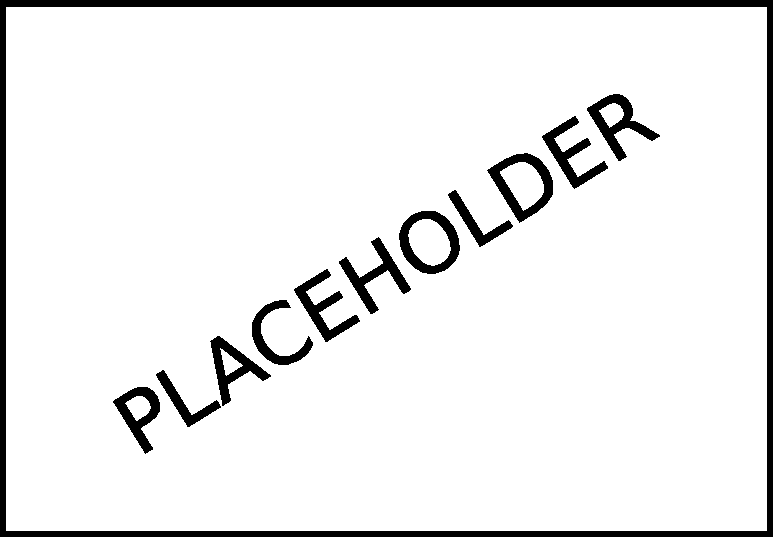
\includegraphics[width=0.8\textwidth]{gfx/placeholder}
    \caption{TODO}\label{fig:connections}
\end{figure}

\section{From C/C to ROS}
\label{sec:cnc-ros}
In Section~\ref{sec:cnc} we already highlighted parallels between the \textit{component-and-connector} paradigm and ROS. At first, it may seem the architectural model of ROS is more complex than a simple component-based approach, since, together with the nodes, there is the extra element of topics, an apparently independent and additional factor. However, topics are nothing more than an agreed name to establish a connection between nodes, they are defined and treated as existing entities in the computational graph, but they do not mediate any communication. After two nodes agree, through mediation of the ROS master, on a communication channel (\ie, a topic), any consequential exchange of messages happens on a direct connection between the two nodes. This means a topics is an aggregation of point-to-point connections and not a independent component mediating the communications. 

Given the actual nature of nodes and topics, it is possible to say that ROS completely follows a \textit{component-and-connector} paradigm, where the nodes are the components and the topics are an aggregation of one or multiple connectors sharing the same characteristics. Figure~\ref{fig:connections} illustrates how all the possible topic configurations (\ie, \textit{1-1}, \textit{n-1}, \textit{1-n} and \textit{n-n}) can be translated in an AADL-based representation, assuming that all the output ports are data ports and all input ports are event data port. The reason of this choice is to model the behaviour of ROS publishers and subscribers. The former does not produce an event notification when it creates a message, it just circulates them in the graph, therefore it is a simple data port, the latter is triggered by the arrival of new messages and supports queue, for this reasons it needs to be modelled as an event data port. As shown in the figure, the substitution process from a topic representation to a connection-based one is quite straightforward. First we select a topic, then we list all the publisher interacting with it, after removing the topic, we directly connect each publisher to all subscribers of the original topic. 

However, by doing this substitution process one piece of fundamental information is lost. In AADL, each connection and each port requires an unique name, this means that it is impossible to maintain the information that a specific connection is part of the aggregation defining the topic. An easy solution is to give the connections a recognisable name, for example each connection for the topic \texttt{/chatter} can have a name starting with \texttt{chatter\_}, however, easy does not translate to good, since this approach is completely unacceptable, it breaks the model by encoding information in variable names. A more elegant solution compatible with the features of AADL is to declare a new \textit{property set}, in this set, called \texttt{topic\_properties}, it is possible to defined two new properties for connections and features. One property is the \textit{Default\_name}, it applies to ports and subprogram accesses, it is used to specify the name of the topic (or service, for subprogram accesses) defined during the implementation of publishers and subscribers. The other property is \textit{Name}, it applies to connections and, at system level, it can be used characterise connections between processes as part of the same topic. The utility of this property is twofold, not only it capture the information of a connection belonging to a topic, but it can be used to include in the model dynamic renaming of topics typical of ROS.

When introducing the concept of component behaviours, we showed how each behaviour can be represented with a specific ROS functionality, however this does not mean that the relationship is bidirectional. ROS imposes very few restriction to the developer, therefore, while the external interface of a node follows the same behaviours presented in Section~\ref{sec:cnc}, the internal implementation may follow an arbitrary pattern. The basic implementation style of a ROS node is to have a main execution loop that periodically polls subscribers and services and pass them the execution every time a new request arrives, similarly to the \textit{component-and-connector} paradigm we presented, this execution happens in a separate environment, however, it is not independent and parallel, but sequential. Practically, this difference it is not meaningful, the conceptual structure presented by the model is the same and this is just an implementation detail. Nevertheless, it is worth to explore an implementation where the actual execution matches completely the description of the model; this will be discussed more in details in Section~TODO. In summary, \textit{sink} and \textit{reactive} behaviours are related to their counterpart in ROS by a bidirectional relationship. It is not possible to say the same when we consider \textit{source} and \textit{filter} behaviours. For reference, let us take the simplest ROS node with publisher functionalities presented in one of the basic ROS tutorial\footnote{http://wiki.ros.org/ROS/Tutorials/WritingPublisherSubscriber(c++)}. In this example, it is possible to see how it is common practice to define a single execution path where everything (\eg, initialisation, polling, publishing, \etc) happens, while this approach is sustainable for small implementations and node with simple behaviours,  it is not suitable for more complex components. This is especially true when implementing components that express multiple \textit{filter} with memory behaviours, in this cases to ensure maintainability, flexibility and understandability of the design it is necessary to follow an approach more in line with the \textit{component-and-connector} paradigm, where each different input and output is managed by an independent execution path. In summary, given the flexibility of the ROS middleware, it is not possible to guarantee that all the implemented node will follow, internally, the design of the \textit{component-and-connector} paradigm. However, the aim of this work is to provide a general modelling approach that can be used to enhance the existing design practices for robotic software, therefore, we will present a way to model (see Section~\ref{sec:ros-in-aadl}) and implement (see Section~TODO) ROS nodes following a simpler, more flexible, easier to maintain and more robust design aligned with the \textit{component-and-connector} paradigm.

While describing the relationship between component behaviours and ROS node implementations, we introduced a key element of any robotic component: the main execution loop. It is in charge of multiple critical tasks of the component; some examples are initialisation, management of incoming requests, dynamic reconfiguration (when supported), error management, shutdown and clean-up procedures. Its role is very important but it is often left out in the modelling phase because of its implicit nature (often hidden by the framework) as the backbone of the component. Nevertheless, it is very important to include it in the modelling process, because some of its tasks may need to be specialised by the developer (\eg, initialisation, error management, \etc). In ROS, in particular, given the freedom left to the developer, it is critical to model the main execution loop to highlight the different functionalities of the nodes, since, as described before, they are often merged in a single execution path. This is another case where for the sake of creating a more general approach and to enhance the ROS design of nodes we, with our modelling approach, overrode the flexibility of ROS to make the main loop an independent execution path disconnected for any other functionality-related path. In summary, in our model, each ROS node, independently from its behaviour, has an additional thread that manages the core functionalities of the component.

\begin{figure}[t]
    \centering
    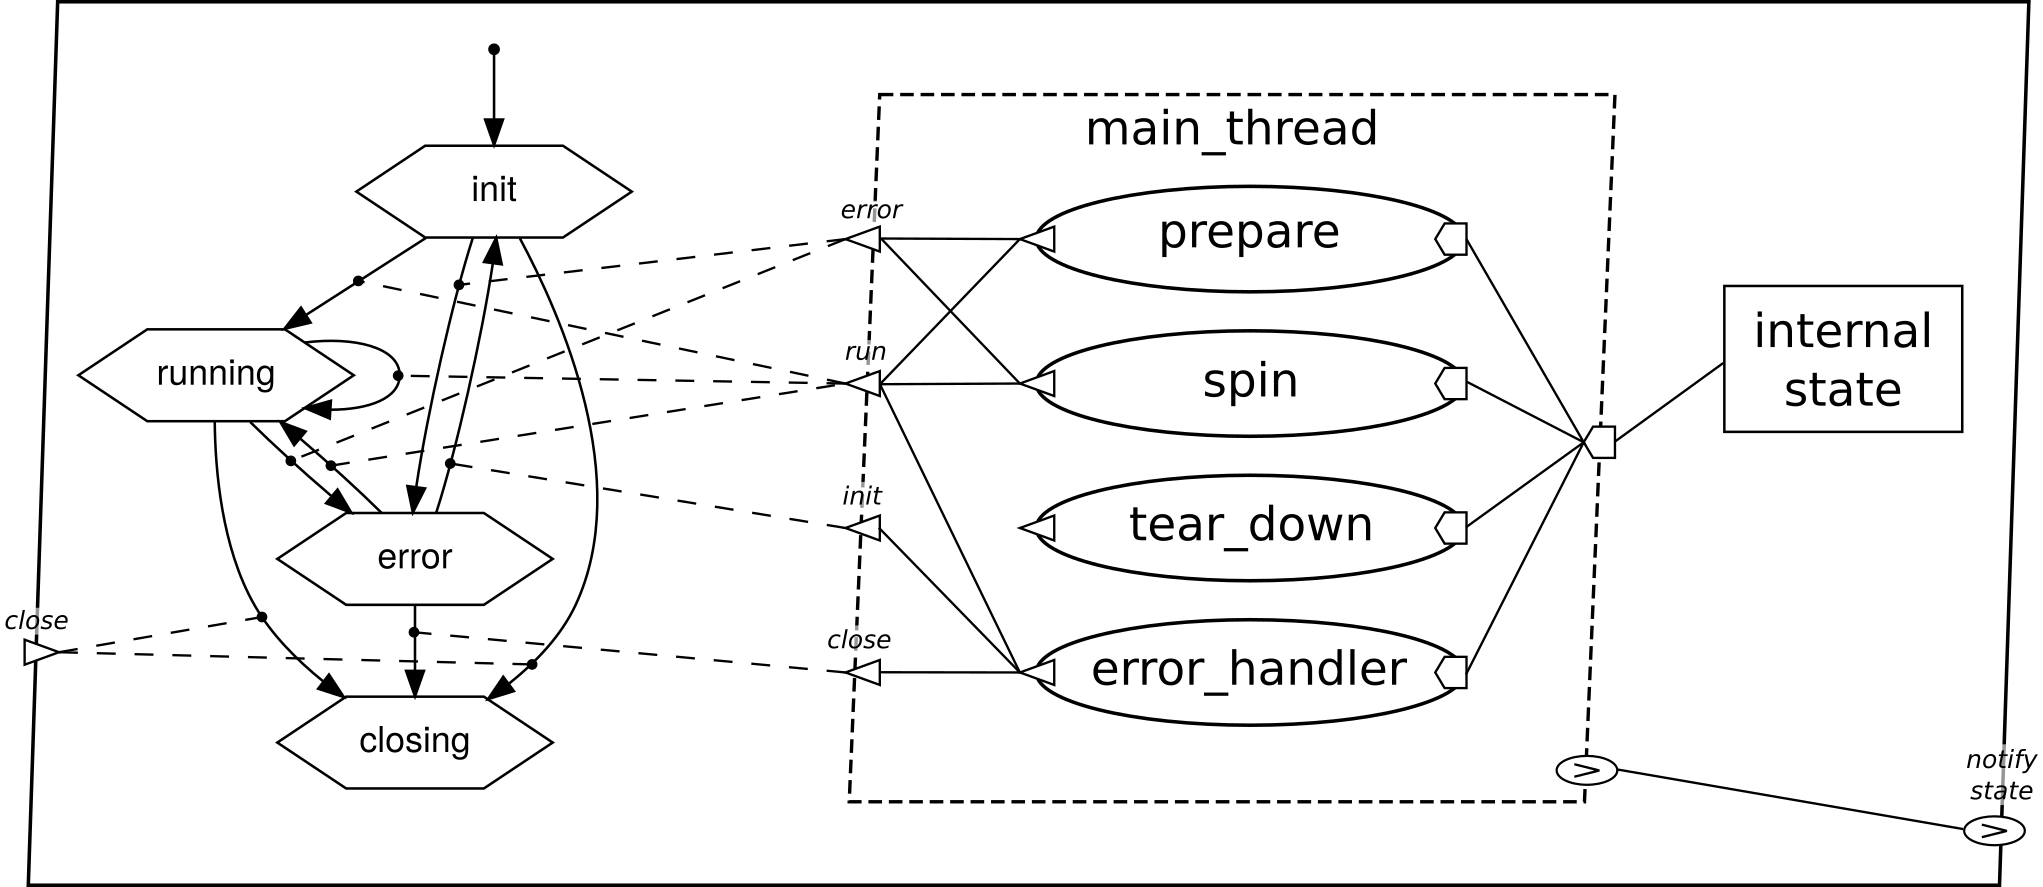
\includegraphics[width=0.95\textwidth]{gfx/essential}
    \caption{TODO}\label{fig:essential}
\end{figure}

\subsection{Modelling a ROS node in AADL}
\label{sec:ros-in-aadl}
In the previous sections, we introduced all the elements we need to model a ROS node: the \textit{component-and-connector} paradigm, how it applies to ROS and the missing elements to bridge from a conceptual model to technological design, and the corresponding AADL description. In this section, we provide a full description of a ROS node, providing first a model of an essential (\ie, no component behaviours) component and then modelling additional functionalities.

Figure~\ref{fig:essential} provides a graphical representation of an essential ROS node. At first glance, it is clear that the model captures more information than what we described until now: the component contain a state machine that is triggered by multiple event ports, the main execution path is detailed by various internal functionalities, there is a permanent internal state and two new features appears on the frontier of the component. Let us analyse the model in order by starting from the state machine: it is used to model the internal life cycle of the component. In ROS there is no defined evolution of the status of a node, usually it can be in only two different states: not executing and active, and the only way to check the current status is to trigger one of the functionalities of the node (\eg, read a topic). However, it is common in component based approaches to define a clear life cycle of the component, moreover, other robotic middlewares and frameworks have an established evolution of the status of their components (\eg, SmartSoft and Orocos), therefore, modelling the internal state machine is a requirement to guarantee the generality of our approach. Our life cycle follows a quite standard structure with four different states.

\paragraph{Init} Initial state of the the life cycle, all the initialisation procedures happen here. After leaving this state it is guarantee the component is ready to execute all its functionalities. From \textit{init}  the component can transition to \textit{running}, when all the initialisation procedure are completed successfully, \textit{error}, or \textit{closing}.
\paragraph{Running} Normal operational state of the component. In this state all the main functionalities are active and the component is working with no issues. The possible transition are: to \textit{running}, the state machine periodically triggers a self loop to ensure that the component is alive and functional, to \textit{error},  or to \textit{closing}.
\paragraph{Error} The component transitions in this state when it captures known errors. While in this state the component is not in execution and recovery procedure can be activate to correct the errors and transition back to an active state (\ie, \textit{init} and \textit{running}), or if the error is unmanageable or catastrophic, to transition to the \textit{closing} state.
\paragraph{Closing} Final state of the life cycle, all the clean up and shut down procedure happens in this state. The transition to this state is triggered by any shutdown signal (internal or external), or when the nodes encounters a catastrophic error that cannot be recovered and requires the node to shut down.
\medskip

Transitions in the state machine are triggered by event ports on the main execution path of the component and on the external frontier. The event port on the frontier is used to model any external signal used to force the shutdown of the node (\eg, SIGINT signal), it triggers the transition to the \textit{closing} state from all active states. All the ports on the main execution thread represents the normal evolution of the system and are activated every time one of the execution phases of the component finishes or when it encounters an error.

The main execution path of the component is modelled using a periodic thread called \textit{main\_thread}. The thread has four subprograms as subcomponents and they represent the active functionalities during each phase of the life cycle. This relationship can be enforced by AADL, since for each state it is possible to specify exactly which subcomponent is active, therefore, while the \textit{main\_thread} is always enabled, only one of its subprograms is active at any given time. Since each subprogram is in charge of a specific state, they are all connected to their corresponding event port to trigger a transition to the next state. Each subprogram has a specific functionality.

\paragraph{Prepare} It is active in the \textit{init} state. This subprogram is in charge of managing node initialisation; it sets parameters, initialise variables, set up publishers and subscribers, and any other node specific initialisation activity. It is connected to the \textit{run} and \textit{error} event ports, to trigger the two possible transitions related with a successful or unsuccessful initialisation.
\paragraph{Spin} It is active in the \textit{running} state, and here the ROS spinner is implemented. When this subprogram is active the \textit{main\_thread} acts as a coordinator of node behaviours, it checks for incoming events and handles potential errors. Two event ports are controlled by this subprograms: \textit{run}, to trigger the self-transition and keep the component active, \textit{error}, to transition to the \textit{error} state when necessary.
\paragraph{Error\_handler} It is active in the \textit{error} state. Here are implemented all the functionalities to deal with known errors of the component, for example an incorrect initialisation or a malformed message. From the \textit{error} state it is possible to transition to any other state, as a result this subprogram is connected to the \textit{run}, \textit{error}, and \textit{init} ports.
\paragraph{Tear\_down} It is active in the \textit{closing} state. This subprogram implements all the procedures related to node shut down. For example, in some cases a node may need to notify another before shutting down, or it need to gracefully disconnect from a physical device. Since this is the final state of the life cycle, this subprogram is connected to no event port on the thread frontier, even so the corresponding port on the subprogram is still modelled for flexibility and potential future extensions.
\medskip

As a final note on the node life cycle, we have included in the model of this essential node a \textit{requires subprogram access} on the frontier of the \textit{main\_thread} which is connected to its counterpart on the process. This access models a remote function call to notify an external supervisor about the current state of the node and any transition. In this way, not only the component has a clear life cycle that defines the execution phases, but it is possible to monitor the evolution of the status through time and keep track of any unexpected behaviour.

Last element to cover is the \textit{internal\_state}, it is a data component used to model the execution memory of the component. In Section~\ref{sec:cnc}, we described how not all the component behaviours requires a shared memory area, therefore, it should not be necessary to include a data component in an essential node. However, in practice, only the simplest component does not require a persistent internal state, because this shared memory area does not exist only as a way for different thread to exchange information. It stores configuration parameters, error mappings, information for shutdown procedures, \etc, for this reasons, not only it is present in this minimal node, but it directly accessible by all subprograms in the \textit{main\_thread}. Since AADL is not a data modelling language (see Chapter~\ref{ch:AADL}), we will not detail here the inner structure of the \textit{internal\_state}, this topic will be covered in Section~\ref{sec:data}.

After modelling an essential node, and by using it as a starting point, we can now add behaviours and functionalities. Figure~\ref{fig:sample-node} shows a graphical representation of a more complex node expressing two coexisting behaviours: a \textit{filter} with memory, modelled with a combination of a \textit{callback} and a \textit{publisher}, and a \textit{filter} with no memory, defined with a subscriber and a publisher in the same thread and identified by the name \textit{callback\_pub}. As introduced in Section~\ref{sec:cnc-ros}, behaviours are modelled using a combination of thread and corresponding ports. In the figure it possible to see how each thread is characterised by a specific port that evokes its functionality: the \textit{callback} has an input event data port, to receive messages and manage queues, the \textit{publisher} has an output data port, to circulate messages to the rest of the architecture, and the \textit{callback\_pub} is a combination of both and has input and output ports. Each port on the thread frontier is then connected to its counterpart on the process to relay from the inside of the component environment to the outside, or vice versa. What is not visible from the figure is the data components associated to each port. In AADL, it is possible to specify the data type exchanged on a connection, and the model will automatically verify that the ports are compatible. Listing~TODO shows a fragment of AADL code where data components associated to ROS messages are declared and used to specify the data type of an hypothetical publisher and subscriber. More details about ROS messages and their definition in the model will be discussed in Section~\ref{sec:data}.

\begin{figure}[t]
    \centering
    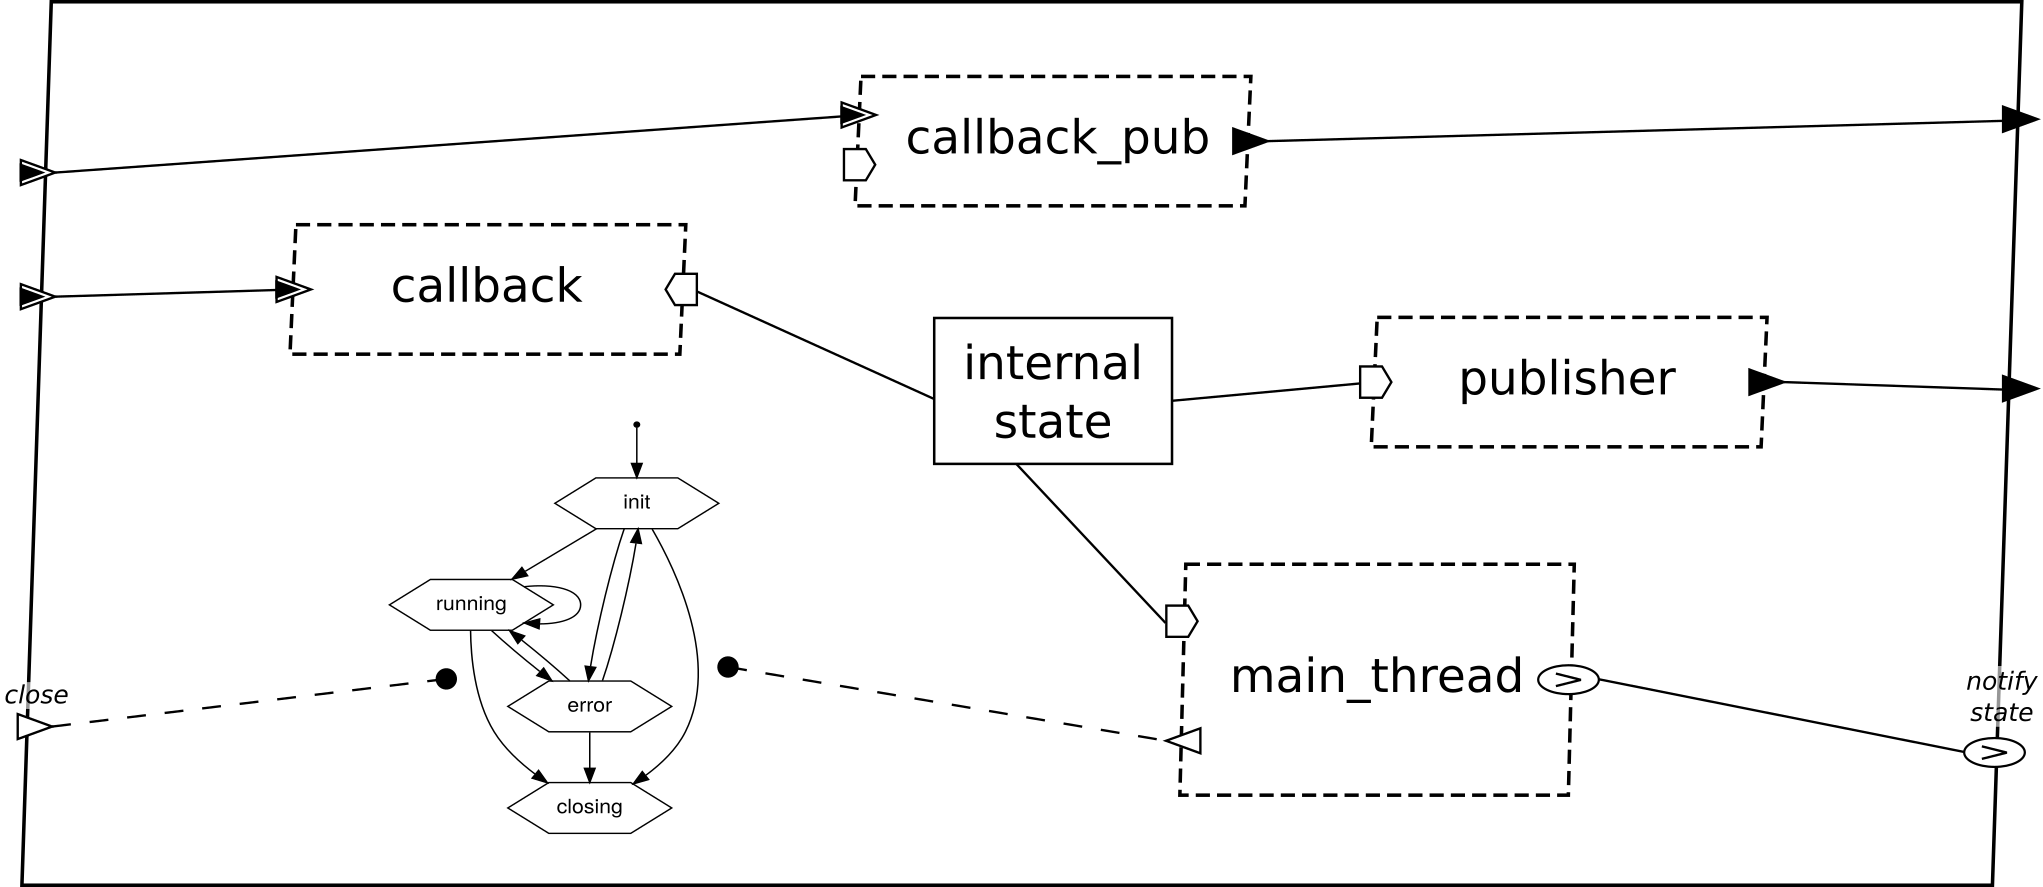
\includegraphics[width=0.95\textwidth]{gfx/sample_node}
    \caption{TODO}\label{fig:sample-node}
\end{figure}

\subsection{Modelling a ROS architecture in AADL}
\label{sec:ros-arch}
In Section~\ref{sec:aadl-robot}, we presented multiple reasons why AADL is a suitable language for robotics, one of them was the capability of the language to model both software and hardware components, however, in our descriptions on how to model ROS nodes we never mentioned any physical interface. The reason for this is that we followed a top down approach to describe a robotic architecture, at higher level of abstraction (\ie, in the \textit{component-and-connector} paradigm) there is no need to make a distinction between a software component and an hardware component, but now that we are moving closer to the actual implementation, this characteristics of AADL will be integrated in our model. We will specify how hardware components can be integrated in the architecture and how to differentiate between communications happening on ROS topic and other physical communication channels. When describing models closer to the implementation level, we also encounter design solutions that are not captured at a more abstract and general level, in ROS there are three key design features that we decided to specifically model in our approach. First of all, existing packages and nodes, the greatest resource of ROS is its repository of already available components, it is imperative to be able to model them correctly in an architecture. Second is \textit{tf}, the coordinates frame manager, it is a backbone of various ROS nodes, therefore it is necessary to include it in the model. Last, it the \textit{actionlib}, an interface to start, monitor, pre-empt and cancel remote tasks, while it is not a commonly used design approach, it is a very useful and elegant way to delegate and coordinate complex task between components.

\paragraph{Physical devices} AADL offers multiple hardware categories to model the physical aspects of a system. For elements like processors or memories we will not go in details, since they work for robotic architectures in the same way of any other, it is possible to bound a software component (\eg, processes or data) to its physical counterpart (\eg, processor and memory) to specify the hardware implementation of the system. In ROS this feature of AADL can be used to model distributed architectures, by binding components to different physical platforms, the designer can specify where each node will be executed at runtime. This creates a deployment view of the system without the need of defining a different model, moreover, AADL analysis capabilities can be used to determine if a specific platform is suitable for a specific subset of the components (\eg, does the target computer has enough RAM to run the system?).

\begin{figure}[t]
    \centering
    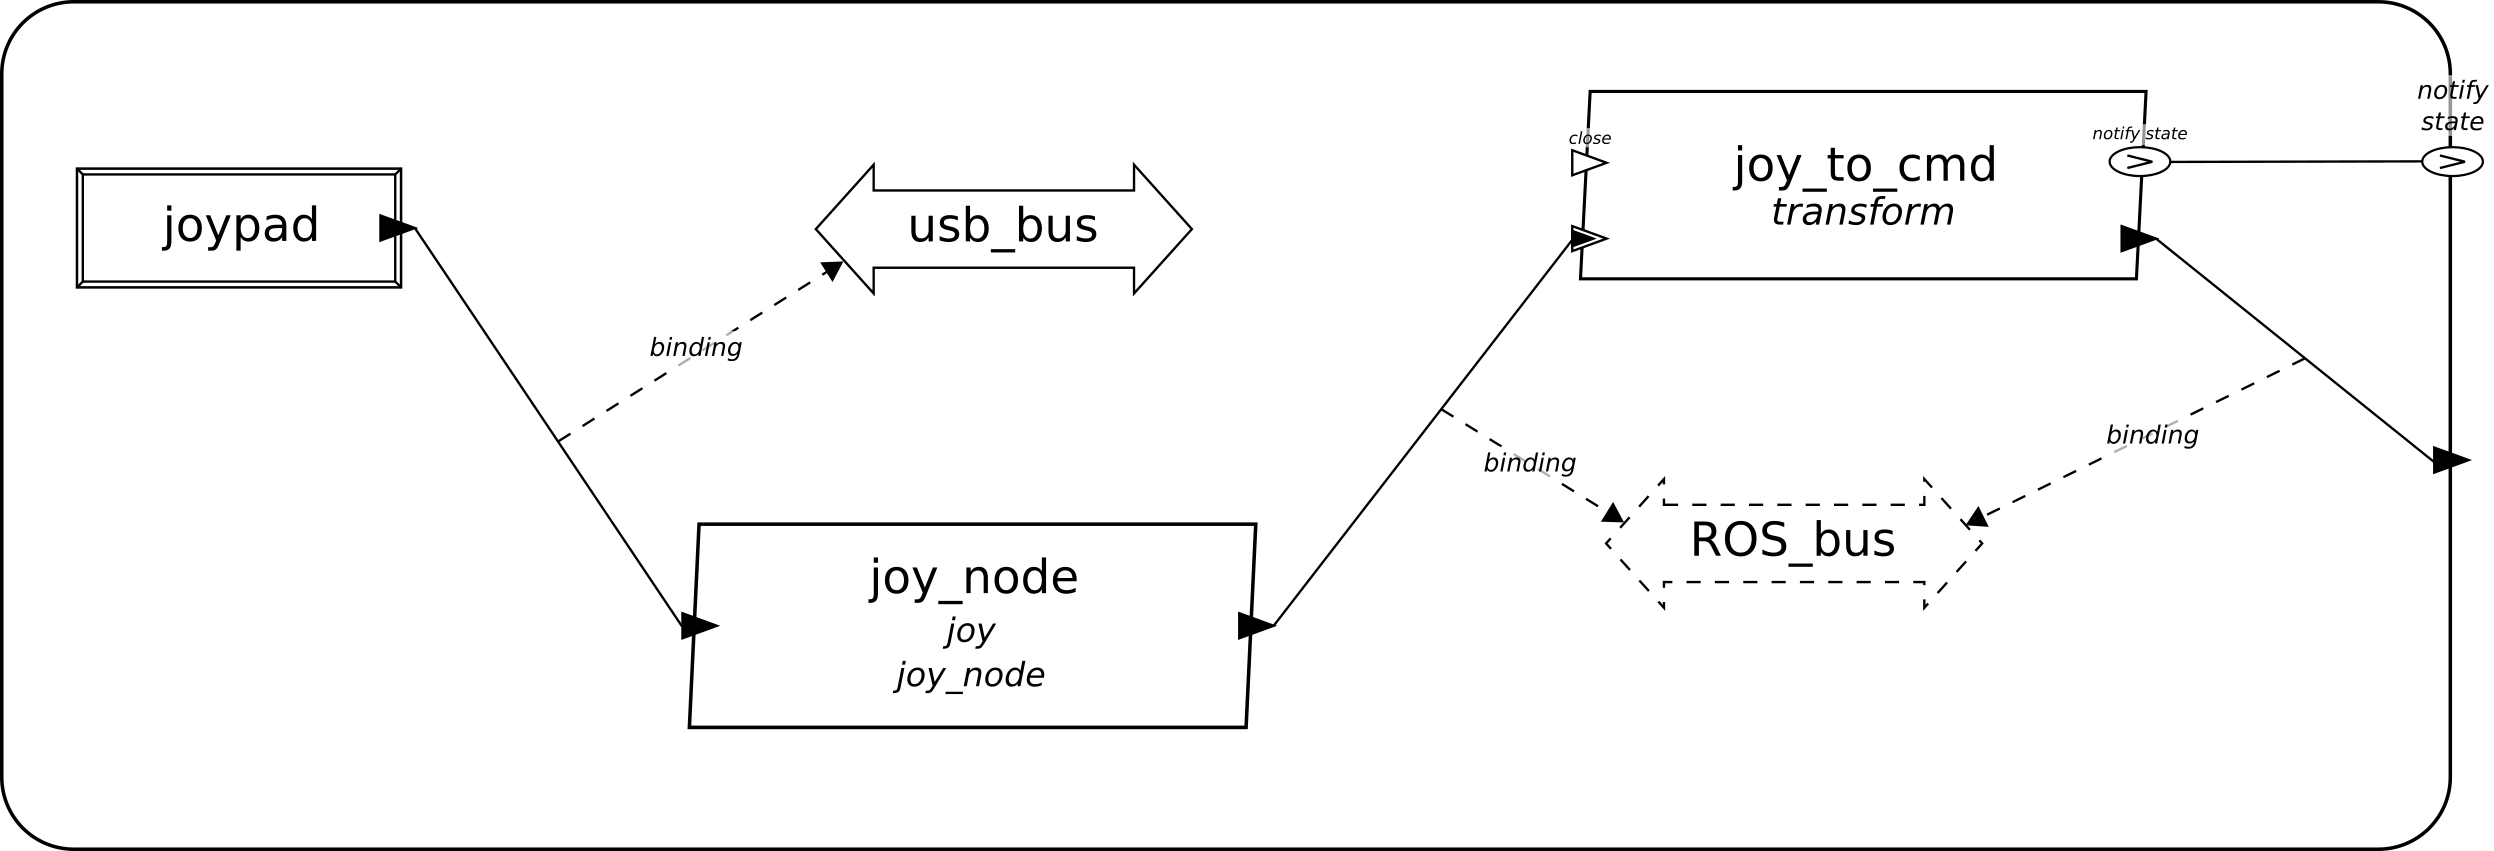
\includegraphics[width=0.95\textwidth]{gfx/mini_arch}
    \caption{TODO}\label{fig:mini-arch}
\end{figure}

What is different in a robotic system is that sensors and actuators are integral part of it, to model them it is possible to use AADL devices. A \textit{device} represents an interface between the physical world and the architecture, it can be modelled as a simple interface or to include the inner functionalities and characteristics of the physical component (\eg, type of communication, computational power, data type).  Devices can connect to processes using ports or accesses, in the same way as processes connect to each other. When modelling a ROS architecture, the fact that physical devices and software components communicate using the same interface rises the issue of differentiate between a topic-based connection and other types of connections; the solution comes in the shape of AADL physical and virtual buses. A \textit{virtual bus} can be used to model abstract communication channels, like ROS topics, while a \textit{bus} can be used for physical connections, like Ethernet and USB. Figure~\ref{fig:mini-arch} shows how this two categories, together with a device, can be used to model a simple joypad-based teleoperation subsystem where a physical bus called \textit{usb\_bus} is bound to the physical connection between the device modelling the joypad and its driver, and a virtual bus called \textit{ROS\_bus} is bound to all the connections representing topics.

\paragraph{Existing ROS nodes} ROS is currently the most popular and widespread robotic middleware, this creates a very prolific and active community, which becomes one of its greatest resources. Given ROS component-based structure and popularity,  a multitude of already existing packages and nodes exist that a developer can simply download and include in his architecture. When creating a modelling approach for ROS it is mandatory to include the possibility to model existing node, to do so we can exploit the dual representation based on component type and implementation provided by AADL.  Existing ROS packages are modelled directly as AADL packages, while existing nodes are modelled using the component type only, basically we provide an interface that appears and behave in the same way as the already existing component, but we do not model in any way the internal functioning. In Figure~\ref{fig:mini-arch}, \textit{joy\_to\_cmd} is a custom made node, completely modelled as visible from the \textit{close} port and the \textit{notify\_state} subprogram access, on the contrary, \textit{joy\_node} is an existing node from the package \textit{joy}, here only topic related ports are modelled to provide an interface to the rest of the system. Listing~TODO shows the textual AADL used to model a ROS packages and node interfaces and how it is then used in an architecture, moreover, it is possible to see how the model descriptions follow the same naming conventions of the original package, while the node name used in the architecture description corresponds to the runtime identifier.

The only potential issue is to create all the models for the existing components, there are few possible solutions that combined can almost automatically generate them. First, analyse the existing nodes at runtime to detect which topics and which messages they use, additionally it is possible to do code inspection to list all the publisher and subscribers, lastly, most packages are documented on the ROS wiki\footnote{http://wiki.ros.org/joy} with, at least, the list and type of topics. Unfortunately, sometimes this is not enough, the joypad driver is one of those example, to detect automatically the connection with the physical device is extremely difficult, at this point the only solution is the human intervention.

\paragraph{tf} This package is one of the core functionalities of ROS and it exists to help manage multiple coordinate frames and transformations over time. Differently from other ROS features, from the point of view of the developer the access to \textit{tf} does not go through any established communication channel (\ie, topics or services), but by using a set of APIs that directly access the distributed coordinate system, additionally, there is no need to start a node to enable it. Therefore, disregarding how \textit{tf} is practically implemented in the system, we can describe it as a centralised resource where all the coordinate frames of the robot and their evolution in time is stored, and it is possible to read or update the content of this shared resource by using specialised APIs. With these assumptions, the best way to model \textit{tf} is to use a single data component at system level that all the nodes can access through data accesses when necessary. The single data component stores the description of the coordinate frames and their evolution in time, while the data accesses represent the bidirectional APIs.

\begin{figure}[t]
    \centering
    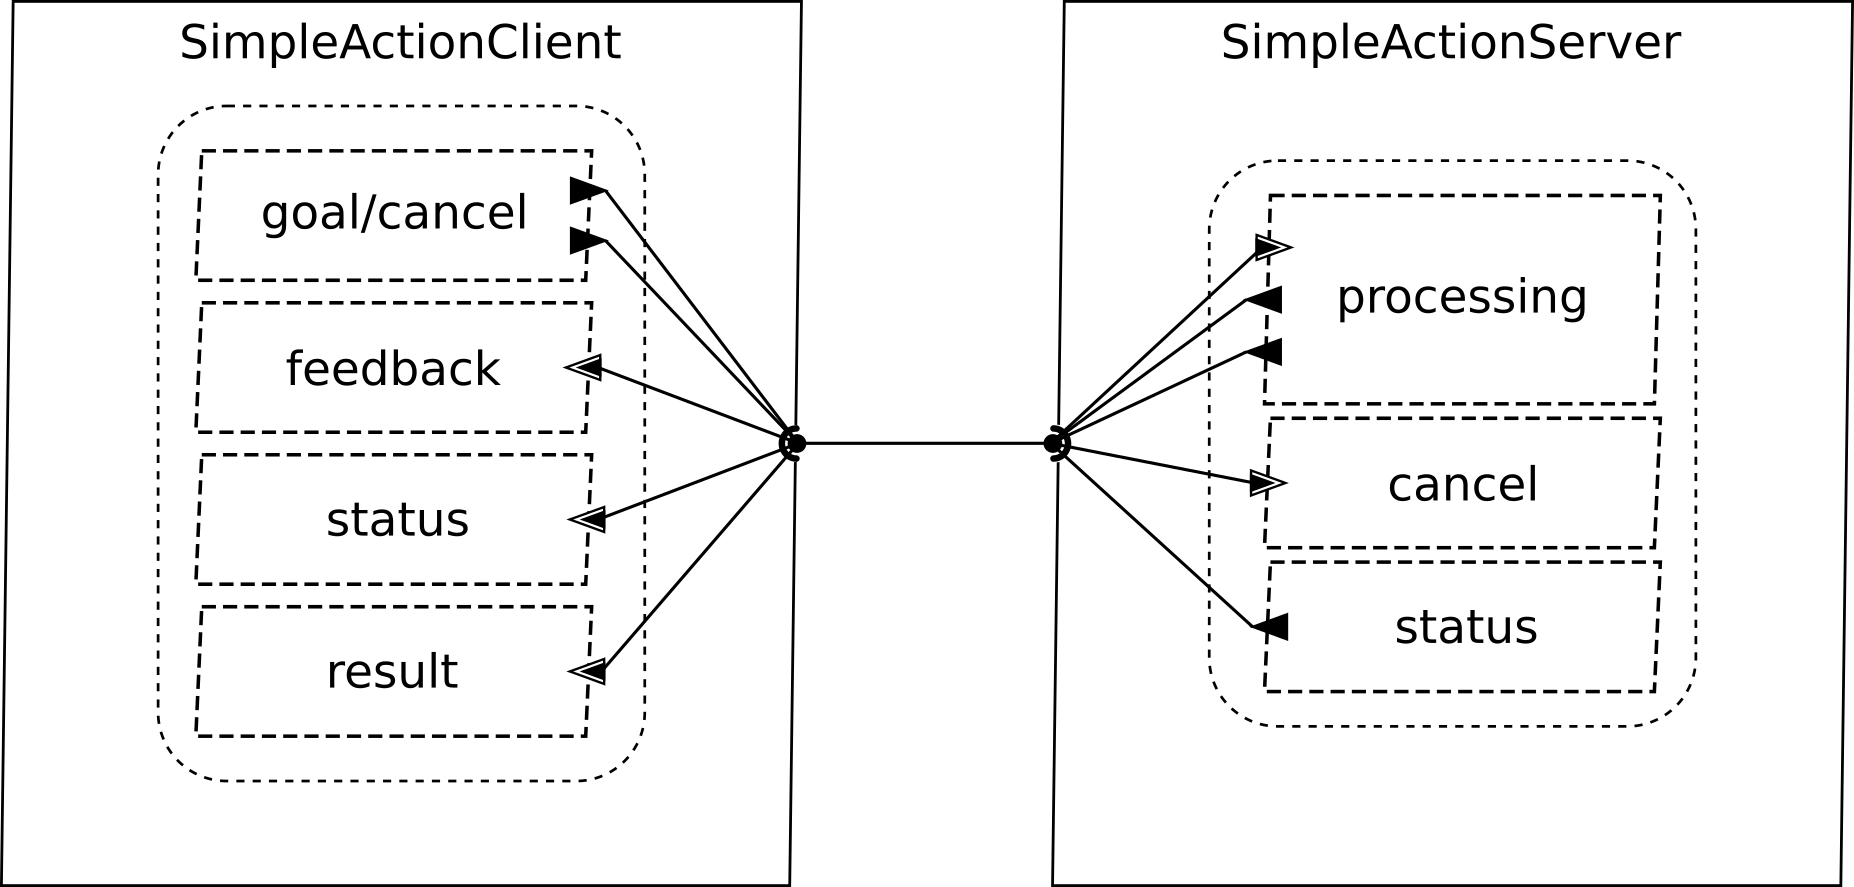
\includegraphics[width=0.95\textwidth]{gfx/action}
    \caption{TODO}\label{fig:action}
\end{figure}

\paragraph{actionlib} Actions are an extension of ROS services, created to manage requests that are too computationally heavy for a traditional client/server approach. An action client can trigger a remote execution on an action server, then resume normal functioning while waiting for a response, if needed. While an action is under execution it sends periodic updates of its status and the original caller can terminate it before it finishes. The actual implementation of ROS actions is based on topics that are used to trigger or cancel the execution, provide the result, and get updates on the status.
% To be able to model correctly an action, it is also necessary to be able to model custom messages, since actions are defined using a \textit{.action} file, which has the same structure of ROS messages, with the difference of being divided in three parts: goal definition, result description and periodic feedback. In our model we use ASN.1 in combination with AADL to do so; the type of the message is defined using a \textit{data} component, in this way AADL syntax will automatically verify the compatibility between the topics, while the actual description of the type it is done using ASN.1, which match the expressive power of the ROS message description language, and, additionally, it provides specification for extra constraints. 
When implementing the action client and server in a ROS node, a developer has to use two already provided classes: \textit{SimpleActionServer} and \textit{SimpleActionClient}. These two classes act as an interface hiding the underlying topic-based system. In AADL it is possible to do the same using a \textit{thread group}; as the name suggest, it is a subcomponent used to group threads together and organize them. Fig.~\ref{fig:action} shows a graphical representation of how an action can be modelled. The client thread group has two outbound ports representing the \textit{goal} topic, used to activate the action, and the \textit{cancel} topic, used to cancel the action; these two ports have their corresponding version on the server group as inbound ports, this time used to trigger the callbacks. The group modelling the \textit{SimpleActionServer} has three outbound ports used to communicate with the client, these ports have their equivalent on the client group. Modelling is about abstracting the underling implementation and representing concepts, therefore at process level the ports of the thread group are aggregated in a \textit{port group}; this maintain the conceptual representation of the action acting as a single communication channel.

\begin{figure}[t]
    \centering
    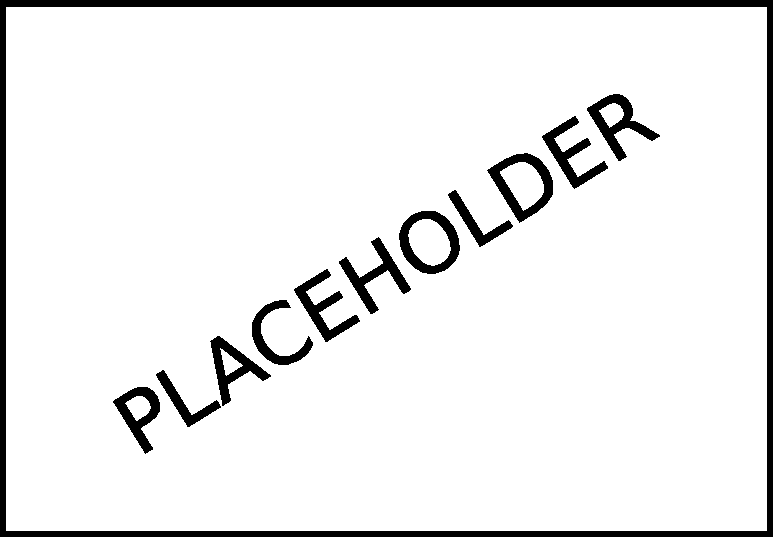
\includegraphics[width=0.8\textwidth]{gfx/placeholder}
    \caption{TODO}\label{fig:ros-arch}
\end{figure}

\subsection{A ROS basic example}
In Section~\ref{sec:cnc-basic}, we presented how to model a simple architecture using AADL and following the \textit{component-and-connector} paradigm. In this section, we describe how that architecture can be updated to represent a complete ROS based system. As visible for Figure~\ref{fig:ros-arch}, the functionalities of the architecture are the same: line following and teleoperation. However, in this updated version, we include ROS specific elements and we model physical components of the system.

Let us start again from the top branch of the architecture: the line following subsystem. From a pure software point of view, the architecture is unchanged, it consists in two components, one expressing a \textit{source} behaviour and the other a \textit{filter} behaviour with no memory. The difference is in the internal representation of the components, now nodes, which is based on the essential node defined in Section~\ref{sec:ros-in-aadl}; it includes the main execution loop, the internal life cycle and the internal state. Both these nodes are assumed to have application specific functionalities, therefore are fully modelled as custom nodes. From an hardware point of view, this subsystem now includes a physical device: the line detection sensor. It is modelled using an AADL device and it has a physical connection with the driver component. The connection is modelled using an output data port on the device and the corresponding input data port on the process, to specify that it does not represent a ROS topic, it is bound to a physical bus that models an USB connection.

The bottom branch is similar to the example presented in Figure~\ref{fig:mini-arch}. On the software side, the teleoperation component is unchanged, but now it is modelled as a ROS node instead of a generic \textit{filter} with memory component, the driver component is replaced by the already existing \textit{joy\_node}, therefore it is modelled only using the external interface. As for the line following subsystem, now the teleoperation subsystem includes the physical device; it models an USB joypad and it is connected to the driver through a data port. Since this connection is a physical UBS connection, too, it is bound to the same physical bus as the connection between the line detector and its driver.

The multiplexer component is now a ROS node. The original \textit{filter} behaviour is now replaced by a set of two subscribers, they collect the messages coming from the two different subsystems, and one publisher, it relays the correct message to the control component. The \textit{reactive} behaviour is implemented using a ROS service, its functionality is the same, an external client can call this service to change the selected input from line following to teleoperation and vice versa.

The control component is now a control subsystem. In the previous version of the architecture, there was a single component expressing a \textit{sink} behaviour, now, the component is replaced by a custom ROS node with a subscriber to receive the set-points and a device modelling the electrical motor. In this case the interaction between the driver and the motor goes through an Ethernet connection, therefore we modelled a second bus component representing this type of connection.

The architecture includes a virtual bus representing ROS topics, all virtual connections (\ie, topics and services) are bound to this bus. While not visible in the figure, the architecture includes data components for message types. Each type is represented by a data component in same package as defined by the existing ROS hierarchy. The data  type of a port is specified in the process definition and port connected together must have the same data type.

\begin{figure}[t]
    \centering
    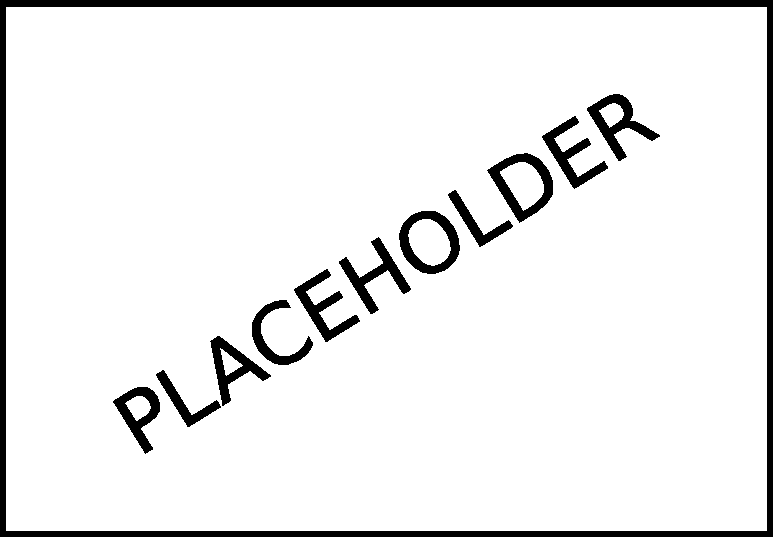
\includegraphics[width=0.8\textwidth]{gfx/placeholder}
    \caption{TODO}\label{fig:template}
\end{figure}

\section{Modelling templates}
With the model definition presented in the previous sections and the ROS-specific models introduced in Section~\ref{sec:ros-arch}, a designer has all the necessary tools to model a functional complete ROS architecture. However, this result does not come without complications, assuming a person is already familiar with AADL, the process of modelling a single architecture is quite tedious and prone to errors, especially replicate the same basic design for all ROS nodes. Moreover, this model aims to be a stepping stone for automatic code generation, for this reason it is necessary the structure of the model is consistent. In summary, there are few issues that need to be addressed:
\begin{enumerate*}[label={\alph*)}]
\item make the modelling approach more accessible, so it can be a reasonable alternative to the current development process for ROS,
\item enforce the presented structure, without it being a burden to the design process,
\item make the underlying structure self-explanatory, without the need of a lengthy accompanied documentation.
\end{enumerate*}

Solving completely all these issue is a very difficult task. In small size project, the process of modelling will always be more complex and time consuming than direct development, until we achieve perfect code generators.  Moreover, there is a limit on how much it is possible to enforce a specific structure, because there is a trade off between the flexibility of an approach and the number of functionality that is possible to model or implement. Nevertheless, in an effort to solve these issues, we developed a series of modelling templates that a designer can use to simplify the modelling process, to do so, we exploited the inheritance capabilities of AADL.

Figure~\ref{fig:template} shows the hierarchy of packages and components when modelling a ROS architecture, and the frontier between the existing templates and the user-created model. At the top of the hierarchy there is the \textit{component-and-connector} paradigm. Here, the main elements of the paradigm are modelled: the component and its implementation, the shared memory area and the inner functionality of behaviours.To model the threads of the behaviours, we used again a hierarchical approach: all behaviour interfaces inherit from the same parent thread which implements the access to the shared memory area as the only common characteristic, then they specify independently their own port to characterise the type of behaviour, only the implementation of the common parent exists since the internal description is always the same (\ie, a single subprogram).

The ROS AADL package extends the \textit{component-and-connector} packages. Here all the necessary elements to model ROS nodes and architectures are defined. The ROS specific elements are modelled directly with no inheritance required, these are: the data component representing \textit{tf}, the virtual bus bound to ROS communications, the main execution loop of the node, and the subprogram associated with the life cycle notification. All the other elements are inherited from the description of the \textit{component-and-connector} package: the node and its implementation extend the component definition, each thread interface extends the corresponding high level behaviour interface (\eg, \textit{service\_provider} extends \textit{reactive}, \textit{callback} extends \textit{sink}, \etc) while the thread implementation extends directly the behaviour implementation. One exception is the ROS timer, since it does not have a corresponding behaviour (it does not interact with the external environment) but it can be used to describe internal functionalities of the node or to give flexibility to the designer, it inherits directly from the general \textit{component\_behaviour} thread. This create the equivalent of a ``ROS node behaviour library''. One element that is necessary to enforce when developing a ROS node is the data type associated with a specific topic, unfortunately the data type of a port is not a mandatory property in AADL. Our solution is to use AADL prototypes; they can be used to create a placeholder for any component or subcomponent. In the thread definition for ROS behaviours, we specified data prototypes associated with the input or output ports, the designer is then forced to specialise them before instantiating the model. Listing~TODO shows how prototypes are defined for the \textit{callback} thread and Listing~TODO shows how they are used in a node definition.

At the lower level of the inheritance there is the specific package to be designed. Other than including the ROS AADL package, it includes all the packages associated with existing ROS nodes and messages. When creating a new node the designer can extend the existing base node provided by the ROS packages, and then add all the necessary functionalities directly from the ROS node behaviour library. This makes the process of modelling a node follow the defined structure, while at the same time, it creates a more compact and easier to design model. Listing~TODO shows how a pair of nodes implementing a publisher and a subscriber can be modelled using this approach.

\section{Data Modelling}
\label{sec:data}
Lorem ipsum

\subsection{ASN.1}
Lorem ipsum

\subsection{JSON}
Lorem ipsum

\subsection{JSON schema}
Lorem ipsum

%*****************************************
